\documentclass[tikz,border=0pt]{standalone}
% Shared look for the README diagrams. Colours are the app's own tokens (web/styles.css).
\usepackage[T1]{fontenc}
\usepackage[scaled=0.95]{helvet}
\renewcommand{\familydefault}{\sfdefault}
\usepackage{amsmath,amssymb}
\usepackage{tikz}
\usetikzlibrary{arrows.meta,positioning,fit,backgrounds,calc,shapes.geometric,shapes.symbols}

\definecolor{ink}{HTML}{15233F}
\definecolor{inksoft}{HTML}{3A4D6B}
\definecolor{paper}{HTML}{D9E7EF}
\definecolor{paperdeep}{HTML}{C6DAE6}
\definecolor{rule}{HTML}{9DB8CB}
\definecolor{safe}{HTML}{17643A}
\definecolor{safewash}{HTML}{D3EBDC}
\definecolor{caution}{HTML}{7A4F00}
\definecolor{cautionwash}{HTML}{F3DFA6}
\definecolor{danger}{HTML}{B0221B}
\definecolor{dangerwash}{HTML}{F7DCD9}
\definecolor{stop}{HTML}{8D0C0C}
\definecolor{stopwash}{HTML}{F6D4CF}
\definecolor{coral}{HTML}{FF8A80}
\definecolor{canvas}{HTML}{F7FAFC}

\newcommand{\modtitle}[1]{{\small\bfseries #1}}
\newcommand{\grouptag}[1]{{\scriptsize\bfseries\color{inksoft}\MakeUppercase{#1}}}

\tikzset{
  every node/.style={font=\footnotesize, text=ink},
  mod/.style={draw=ink, line width=0.7pt, fill=white, rounded corners=3pt, align=center,
              minimum height=1.25cm, inner sep=4pt},
  api/.style={mod, fill=paper},
  actor/.style={mod, fill=ink, text=white, minimum width=2.8cm},
  frame/.style={draw=rule, line width=0.8pt, dashed, rounded corners=6pt, inner sep=10pt},
  flow/.style={-{Stealth[length=6pt,width=5pt]}, line width=0.8pt, draw=ink},
  soft/.style={flow, draw=inksoft, dashed},
  halo/.style={preaction={draw=canvas, line width=4pt, -}},
  lab/.style={font=\scriptsize, text=inksoft, fill=canvas, inner sep=1.5pt},
  store/.style={cylinder, shape border rotate=90, aspect=0.18, draw=ink, line width=0.7pt,
                fill=paper, align=center, minimum height=1.35cm, inner sep=4pt},
}

% Light card behind everything (own layer, under the frames), so the SVG reads on GitHub's dark theme too.
\pgfdeclarelayer{card}
\pgfsetlayers{card,background,main}
\newcommand{\card}{%
  \begin{pgfonlayer}{card}
    \fill[canvas, rounded corners=10pt]
      ($(current bounding box.south west)+(-0.5,-0.5)$) rectangle ($(current bounding box.north east)+(0.5,0.5)$);
  \end{pgfonlayer}}
% code names without a bitmap typewriter font
\newcommand{\code}[1]{{\color{inksoft}\itshape #1}}
\begin{document}
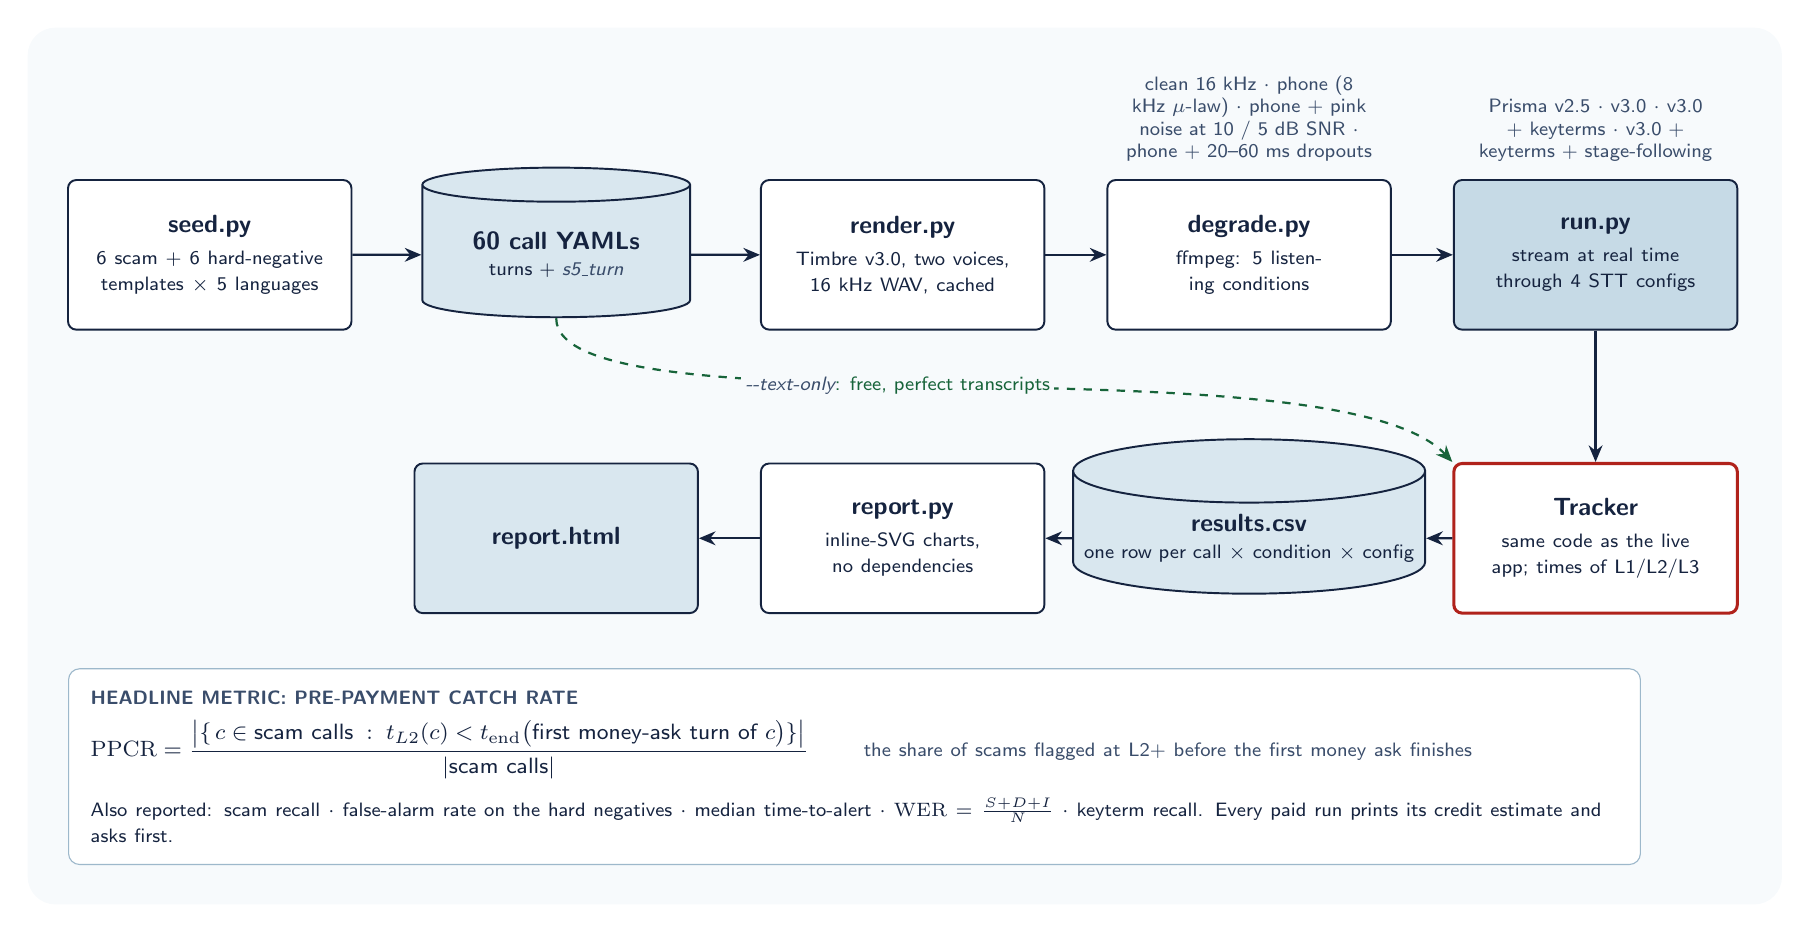
\begin{tikzpicture}[x=1cm,y=1cm,
  stage/.style={mod, minimum width=3.6cm, minimum height=1.9cm, text width=3.3cm},
  note/.style={font=\scriptsize, text=inksoft, align=center, text width=3.5cm}]

\node[stage] (seed)  at (0,0)    {\modtitle{seed.py}\\[2pt]{\scriptsize 6 scam + 6 hard-negative templates $\times$ 5 languages}};
\node[store, minimum width=3.4cm, minimum height=1.9cm] (calls) at (4.4,0) {\modtitle{60 call YAMLs}\\{\scriptsize turns + \code{s5\_turn}}};
\node[stage] (render) at (8.8,0) {\modtitle{render.py}\\[2pt]{\scriptsize Timbre v3.0, two voices, 16 kHz WAV, cached}};
\node[stage] (degr)  at (13.2,0) {\modtitle{degrade.py}\\[2pt]{\scriptsize ffmpeg: 5 listening conditions}};
\node[stage, fill=paperdeep] (run) at (17.6,0) {\modtitle{run.py}\\[2pt]{\scriptsize stream at real time through 4 STT configs}};
\node[stage, draw=danger, line width=1.1pt] (trk) at (17.6,-3.6) {\modtitle{Tracker}\\[2pt]{\scriptsize same code as the live app; times of L1/L2/L3}};
\node[store, minimum width=3.4cm, minimum height=1.9cm] (csv) at (13.2,-3.6) {\modtitle{results.csv}\\{\scriptsize one row per call $\times$ condition $\times$ config}};
\node[stage] (rep) at (8.8,-3.6) {\modtitle{report.py}\\[2pt]{\scriptsize inline-SVG charts, no dependencies}};
\node[stage, fill=paper] (html) at (4.4,-3.6) {\modtitle{report.html}};

\foreach \a/\b in {seed/calls, calls/render, render/degr, degr/run, run/trk, trk/csv, csv/rep, rep/html} \draw[flow] (\a) -- (\b);
\draw[flow, dashed, draw=safe] (calls.south) .. controls +(0,-1.5) and +(-1.5,1.6) .. node[lab, pos=0.45, text=safe, fill=canvas] {\code{-{}-text-only}: free, perfect transcripts} (trk.north west);

\node[note, above=3pt of degr] {clean 16 kHz $\cdot$ phone (8 kHz $\mu$-law) $\cdot$ phone + pink noise at 10 / 5 dB SNR $\cdot$ phone + 20--60 ms dropouts};
\node[note, above=3pt of run] {Prisma v2.5 $\cdot$ v3.0 $\cdot$ v3.0 + keyterms $\cdot$ v3.0 + keyterms + stage-following};

% ---- metrics -------------------------------------------------------------------------
\node[draw=rule, fill=white, rounded corners=4pt, inner sep=8pt, anchor=north west, text width=19.4cm] at (-1.8,-5.25) {%
  \grouptag{Headline metric: Pre-Payment Catch Rate}\\[5pt]
  $\displaystyle \mathrm{PPCR}=\frac{\bigl|\{\,c\in\text{scam calls} \;:\; t_{L2}(c) < t_{\mathrm{end}}\bigl(\text{first money-ask turn of } c\bigr)\}\bigr|}{|\text{scam calls}|}$
  \qquad {\scriptsize\color{inksoft}the share of scams flagged at L2+ before the first money ask finishes}\\[6pt]
  {\scriptsize Also reported: scam recall $\cdot$ false-alarm rate on the hard negatives $\cdot$ median time-to-alert $\cdot$
   $\mathrm{WER}=\frac{S+D+I}{N}$ $\cdot$ keyterm recall. Every paid run prints its credit estimate and asks first.}};

\card
\end{tikzpicture}
\end{document}
